% =========================================================================
% LaTeX figure snippets for Chapter 4 final figures
% Generated by scripts/generate_results_final_figures.py
%
% Recommended main chapter figures: A (01), 01b (conditional), B (02), C (03), E (05)
% Appendix figures:                 D (04), F (06)
%
% Usage: place \graphicspath{{figs/results_final/}} in preamble, or use
% full relative paths as shown below.
% =========================================================================

% -------------------------------------------------------------------------
% Figure A — Pre-retrieval NDCG by representation  (§4.2)
% -------------------------------------------------------------------------
\begin{figure}[htbp]
  \centering
  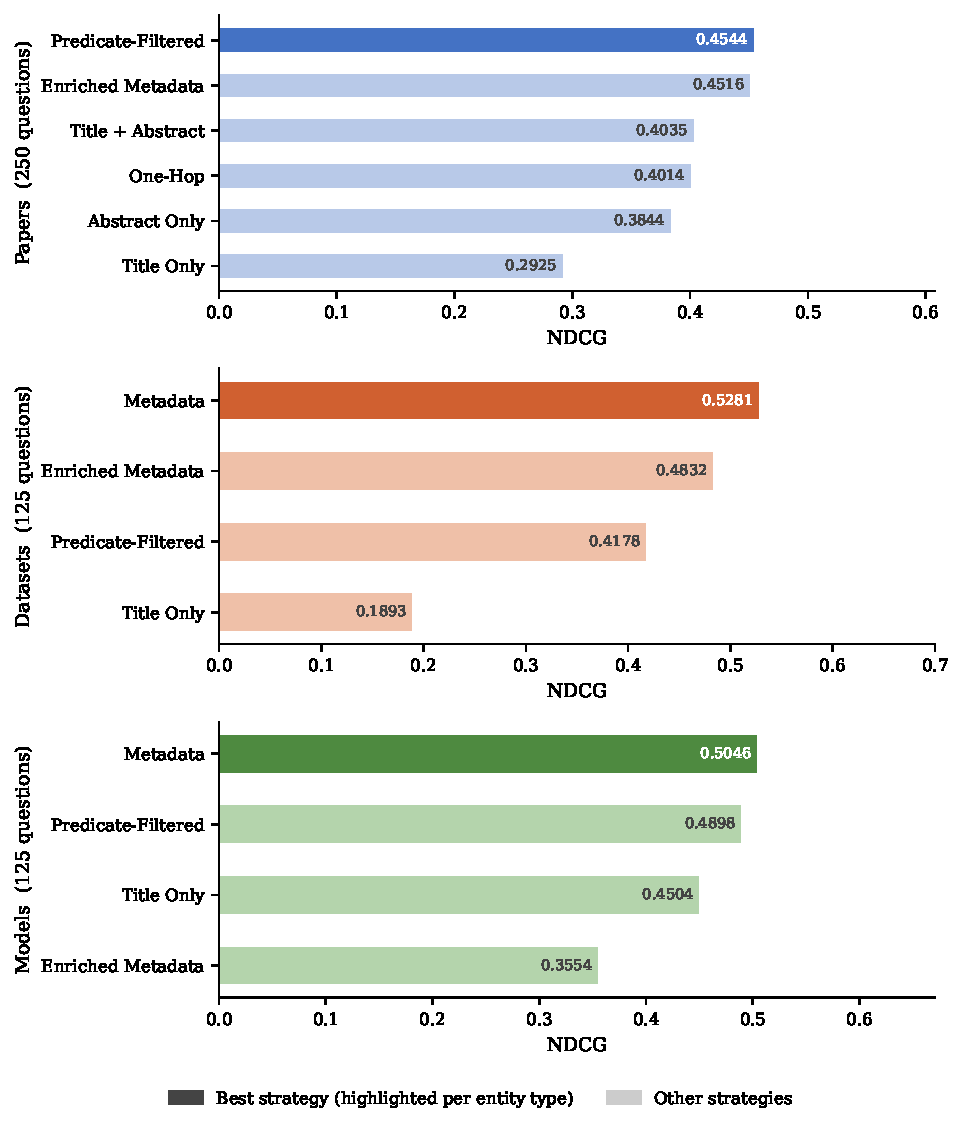
\includegraphics[width=\linewidth]{figs/results_final/01_pre_retrieval_ndcg_by_representation.pdf}
  \caption{%
    NDCG scores for all evaluated textual representation strategies, grouped by
    entity type. Each panel shows representations ordered by NDCG from lowest to
    highest; the highest-scoring strategy per entity type is highlighted.
    Best strategies: Predicate-Filtered for papers (NDCG\,=\,0.4544),
    Metadata for datasets (NDCG\,=\,0.5281), and Metadata for models
    (NDCG\,=\,0.5046). Evaluated on 500 answerable questions (250 paper,
    125 dataset, 125 model).
  }
  \label{fig:pre_retrieval_ndcg_by_representation}
\end{figure}

% -------------------------------------------------------------------------
% Figure 01b — Pre-retrieval NDCG by entity type × difficulty  (§4.2)
% Optional main-chapter figure — use if §4.2 contains a Difficulty and
% Question-Type Analysis subsection; otherwise place in appendix.
% -------------------------------------------------------------------------
\begin{figure}[htbp]
  \centering
  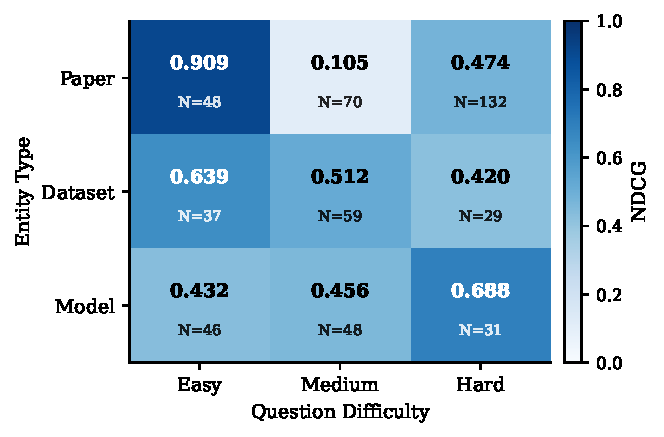
\includegraphics[width=0.68\linewidth]{figs/results_final/01b_pre_retrieval_ndcg_by_entity_difficulty.pdf}
  \caption{%
    NDCG of the selected best representation per entity type across question
    difficulty levels. Best representations: Predicate-Filtered (papers),
    Metadata (datasets and models). N indicates the number of evaluable questions
    per entity-type and difficulty combination. Easy questions consistently yield
    higher NDCG across all entity types; medium questions are the weakest
    segment, particularly for papers (NDCG\,=\,0.NNN).
  }
  \label{fig:pre_retrieval_ndcg_by_entity_difficulty}
\end{figure}

% -------------------------------------------------------------------------
% Figure B — Retrieval method comparison  (§4.3)
% -------------------------------------------------------------------------
\begin{figure}[htbp]
  \centering
  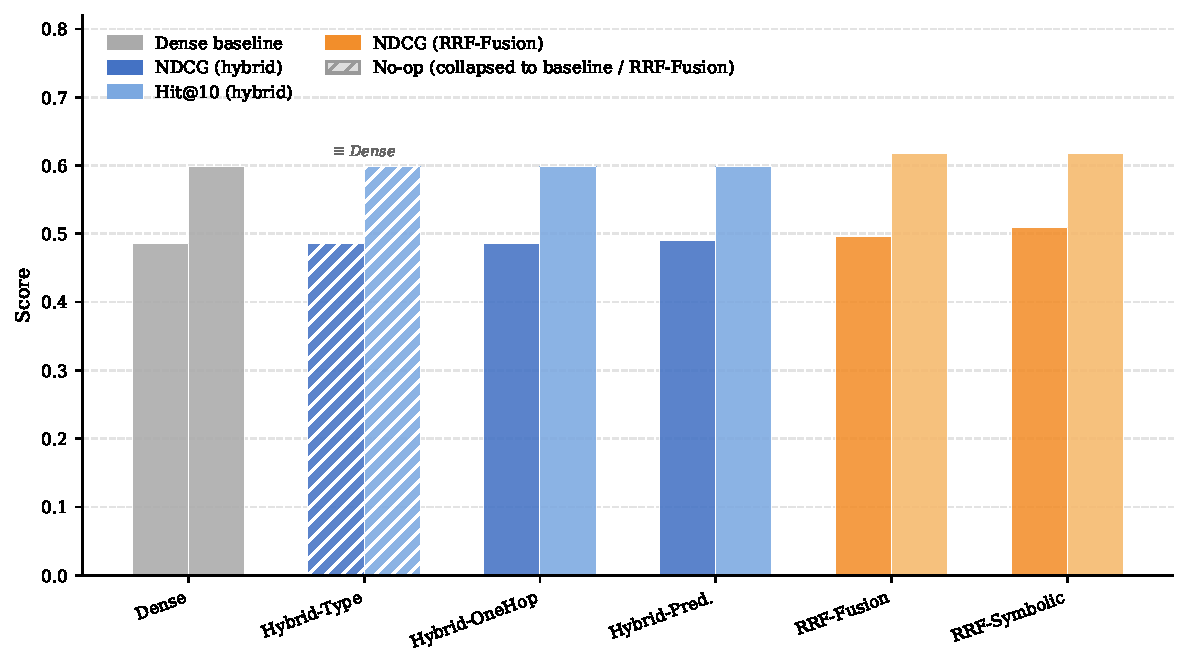
\includegraphics[width=\linewidth]{figs/results_final/02_retrieval_method_comparison.pdf}
  \caption{%
    NDCG and Hit@10 scores for all six retrieval methods.
    Hatched bars (\(\equiv\) annotations) indicate methods that are
    implementation no-ops: Hybrid-Type and Hybrid-Predicate produce output
    identical to the Dense baseline; RRF-Symbolic produces output identical
    to RRF-Fusion. The only genuine improvements over the Dense baseline are
    Hybrid-OneHop (marginal) and RRF-Fusion (Hit@10 +0.020, NDCG +0.011).
  }
  \label{fig:retrieval_method_comparison}
\end{figure}

% -------------------------------------------------------------------------
% Figure C — Question-type NDCG heatmap  (§4.3)
% -------------------------------------------------------------------------
\begin{figure}[htbp]
  \centering
  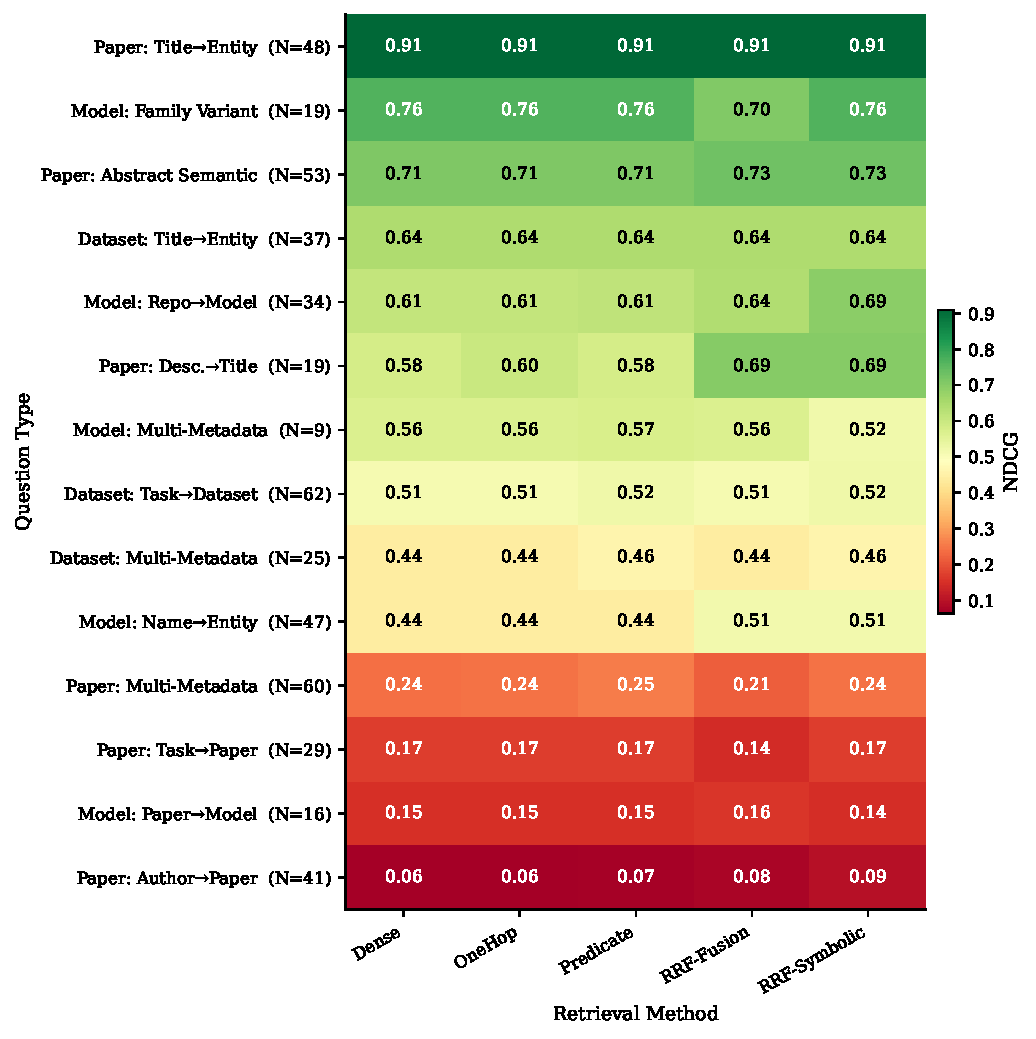
\includegraphics[width=\linewidth]{figs/results_final/03_retrieval_question_type_heatmap.pdf}
  \caption{%
    NDCG by question type for the three behaviourally distinct retrieval
    methods. Rows are sorted by Dense baseline NDCG (descending); N gives the
    number of questions per type. High-confidence title-lookup questions
    (\emph{Title$\to$Entity}) reach NDCG $>$ 0.90, while low-resource
    multi-hop types (\emph{Task$\to$Paper}, \emph{Author$\to$Paper}) remain
    below 0.20 across all methods.
  }
  \label{fig:retrieval_question_type_heatmap}
\end{figure}

% -------------------------------------------------------------------------
% Figure E — Retrieval NDCG by difficulty  (§4.3)
% -------------------------------------------------------------------------
\begin{figure}[htbp]
  \centering
  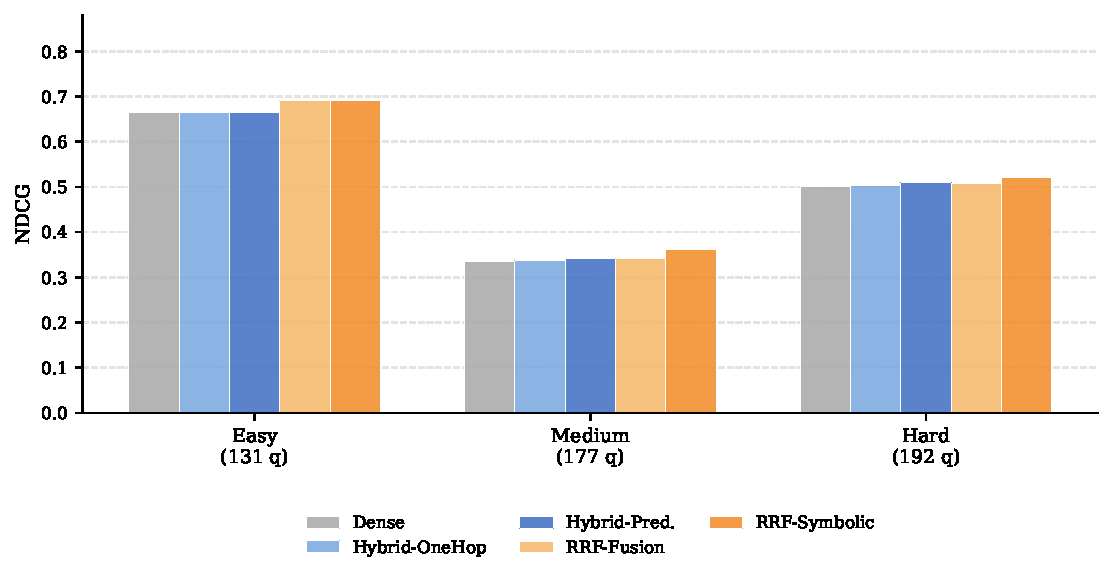
\includegraphics[width=0.85\linewidth]{figs/results_final/05_retrieval_ndcg_by_difficulty.pdf}
  \caption{%
    NDCG broken down by question difficulty for the three behaviourally
    distinct retrieval methods. Easy questions benefit most from RRF-Fusion
    (NDCG\,=\,0.6904 vs.\ 0.6652 for Dense). Medium questions remain the
    weakest segment (NDCG\,$\leq$\,0.34) across all methods, indicating that
    multi-constraint queries present a persistent retrieval challenge
    independent of the ranking strategy.
  }
  \label{fig:retrieval_ndcg_by_difficulty}
\end{figure}

% =========================================================================
% Appendix figures (D and F) — include below if needed
% =========================================================================

% Figure D — Entity-type NDCG heatmap  (Appendix)
% \begin{figure}[htbp]
%   \centering
%   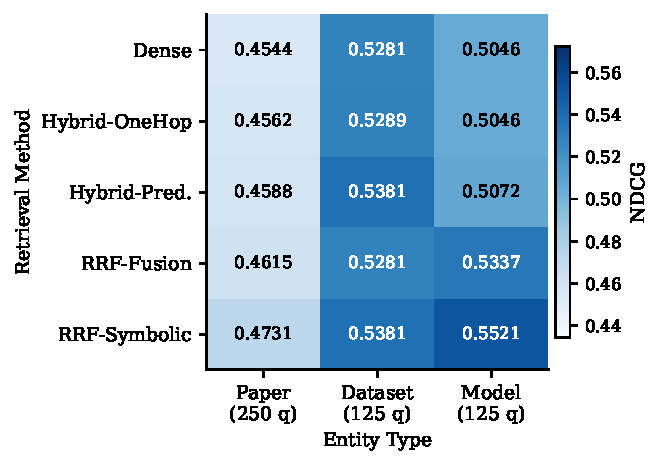
\includegraphics[width=0.65\linewidth]{figs/results_final/04_retrieval_ndcg_by_entity_type.pdf}
%   \caption{%
%     NDCG by entity type for the three distinct retrieval methods.
%     Dataset retrieval benefits least from RRF-Fusion, while model retrieval
%     shows the largest gain (+0.029 NDCG over Dense).
%   }
%   \label{fig:retrieval_ndcg_by_entity_type}
% \end{figure}

% Figure F — Hit@1 vs Hit@10 gap  (Appendix)
% \begin{figure}[htbp]
%   \centering
%   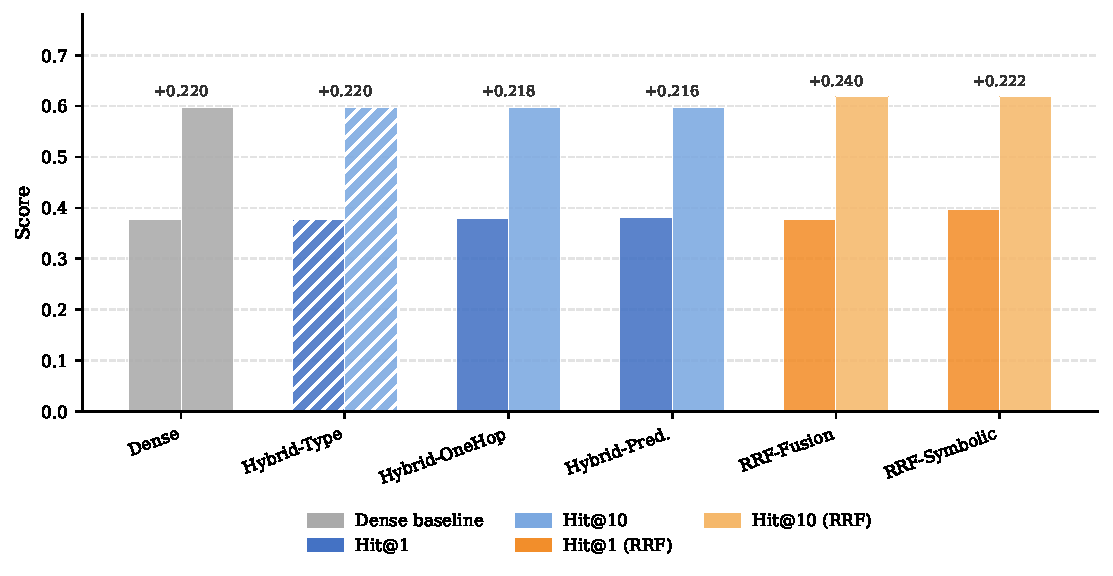
\includegraphics[width=\linewidth]{figs/results_final/06_retrieval_hit_gap_optional.pdf}
%   \caption{%
%     Hit@1 and Hit@10 for all six retrieval methods, with the recoverability
%     gap annotated above each pair. The gap is consistent across methods
%     (0.218--0.240), confirming that ranking position within the top-10 window
%     is the main differentiating factor rather than the presence or absence of
%     the gold entity in the candidate list.
%   }
%   \label{fig:retrieval_hit_gap}
% \end{figure}
